\usepackage[utf8]{inputenc}
\usepackage{graphicx, epsfig}
\usepackage{amsmath,mathrsfs,amsfonts,amssymb}
\usepackage{floatflt}
\usepackage{epic,ecltree}
\usepackage{mathtext}
\usepackage{fancybox}
\usepackage{fancyhdr}
\usepackage{multirow}
\usepackage{enumerate}
\usepackage{epstopdf}
\usepackage{multicol}
\usepackage{algorithm}
\usepackage[noend]{algorithmic}
\usepackage{tikz}
\usepackage{blindtext}
\usepackage{multido}
\usetheme{default}%{Singapore}%{Warsaw}%{Warsaw}%{Darmstadt}
\usecolortheme{default}

\setbeamerfont{title}{size=\Huge}
\setbeamertemplate{footline}[frame number]{}

\setbeamertemplate{section in toc}[sections numbered]

\makeatletter
\newcommand\HUGE{\@setfontsize\Huge{35}{40}}
\makeatother    

\setbeamerfont{title}{size=\HUGE}
\beamertemplatenavigationsymbolsempty

\usetikzlibrary{arrows,shapes,positioning,shadows,trees}

\newcommand\myfootnote[1]{%
  \vspace{-0.5cm}%
  \tikz[remember picture,overlay]
  \draw (current page.south west) +(1in + \oddsidemargin,0.5em)
  node[anchor=south west,inner sep=0pt]{\parbox{\textwidth}{%
      \rlap{\rule{10em}{0.4pt}}\raggedright\scriptsize \textit{#1}}};}

\newcommand\myfootnotewithlink[2]{%
  \vspace{-0.5cm}%
  \tikz[remember picture,overlay]
  \draw (current page.south west) +(1in + \oddsidemargin,0.5em)
  node[anchor=south west,inner sep=0pt]{\parbox{\textwidth}{%
      \rlap{\rule{10em}{0.4pt}}\raggedright\scriptsize\href{#1}{\textit{#2}}}};}

\AtBeginSection[]
      {
      	\begin{frame}{Outline}
      		\tableofcontents[currentsection]
      	\end{frame}
      }
      \AtBeginSubsection[]{
      	\begin{frame}{Outline}
      		\tableofcontents[currentsection,currentsubsection]
      	\end{frame}
}

\newcounter{noscounter} % Используется для nextonslide команды (обнуляется только на новом слайде)
\newcounter{pcounter} % Используется для pause команды (обнуляется после использования eqpause)
\newcounter{diffcounter} % Считает количество pause после формулы

\newcommand{\nextonslide}[1]{%
  \stepcounter{noscounter}% Прибавляем счетчик nextonslide
  \stepcounter{pcounter}% Прибавляем счетчик pause
  \stepcounter{diffcounter}% Прибавляем счетчик diffcounter
  \onslide<\value{noscounter}->{#1}% Отображаем аргумент в скобках на слайде с номером noscounter
}
\newcommand{\resetonslide}{%
    \setcounter{noscounter}{1}% Сбрасываем счетчик nextonslide
    \setcounter{pcounter}{1}% Сбрасываем счетчик pause
    \setcounter{diffcounter}{0}% Сбрасываем счетчик diffcounter
}

\newcommand{\eqpause}{%
  \multido{\i=1+1}{\value{pcounter}}{\pause}% Повторяем pcounter раз команду pause
  \stepcounter{noscounter}% Прибавляем счетчик nextonslide
  \setcounter{pcounter}{1}% Сбрасываем счетчик pause
}

\newcommand{\eqpausediff}{% Вспомогательная команда, запускается автоматически после формул
  \multido{\i=1+1}{\value{diffcounter}}{\pause}% Повторяем diffcounter раз команду pause
  \addtocounter{pcounter}{-\value{diffcounter}}% Вычитаем из pcounter количество сделанных pause
  \setcounter{diffcounter}{0}% Сбрасываем счетчик diffcounter
}

\newcommand\AtEndBoth[2]{% Применяем команду к multline и multline*
  \AtEndEnvironment{#1}{#2}%
  \AtEndEnvironment{#1*}{#2}%
}

\AtEndBoth{align}{\eqpausediff}
\AtEndBoth{equation}{\eqpausediff}
\AtEndBoth{multline}{\eqpausediff}

\addtobeamertemplate{frametitle}{\resetonslide}{}% На каждом слайде сбрасываем счетчики

% latin bold lower
\newcommand{\ba}{\mathbf{a}} 
\newcommand{\bc}{\mathbf{c}} 
\newcommand{\be}{\mathbf{e}} 
\newcommand{\bff}{\mathbf{f}} % \bf - for bold type
\newcommand{\bg}{\mathbf{g}} 
\newcommand{\bh}{\mathbf{h}} 
\newcommand{\bp}{\mathbf{p}} 
\newcommand{\bq}{\mathbf{q}} 
\newcommand{\bt}{\mathbf{t}} 
\newcommand{\bs}{\mathbf{s}} 
\newcommand{\bu}{\mathbf{u}} 
\newcommand{\bv}{\mathbf{v}} 
\newcommand{\bw}{\mathbf{w}} 
\newcommand{\bx}{\mathbf{x}} 
\newcommand{\by}{\mathbf{y}} 
\newcommand{\bz}{\mathbf{z}} 

% latin bold upper
\newcommand{\bA}{\mathbf{A}} 
\newcommand{\bB}{\mathbf{B}} 
\newcommand{\bC}{\mathbf{C}} 
\newcommand{\bG}{\mathbf{G}} 
\newcommand{\bI}{\mathbf{I}} 
\newcommand{\bJ}{\mathbf{J}} 
\newcommand{\bL}{\mathbf{L}} 
\newcommand{\bM}{\mathbf{M}} 
\newcommand{\bP}{\mathbf{P}}
\newcommand{\bQ}{\mathbf{Q}} 
\newcommand{\bR}{\mathbf{R}} 
\newcommand{\bT}{\mathbf{T}} 
\newcommand{\bU}{\mathbf{U}} 
\newcommand{\bV}{\mathbf{V}} 
\newcommand{\bW}{\mathbf{W}} 
\newcommand{\bX}{\mathbf{X}} 
\newcommand{\bY}{\mathbf{Y}} 
\newcommand{\bZ}{\mathbf{Z}} 

% latin cal upper
\newcommand{\cF}{\mathcal{F}} 
\newcommand{\cG}{\mathcal{G}} 
\newcommand{\cI}{\mathcal{I}} 
\newcommand{\cL}{\mathcal{L}} 
\newcommand{\cM}{\mathcal{M}} 
\newcommand{\cN}{\mathcal{N}} 
\newcommand{\cP}{\mathcal{P}} 
\newcommand{\cS}{\mathcal{S}} 
\newcommand{\cT}{\mathcal{T}} 
\newcommand{\cW}{\mathcal{W}} 
\newcommand{\cX}{\mathcal{X}} 
\newcommand{\cZ}{\mathcal{Z}} 

% latin bb upper
\newcommand{\bbE}{\mathbb{E}} 
\newcommand{\bbI}{\mathbb{I}} 
\newcommand{\bbP}{\mathbb{P}} 
\newcommand{\bbR}{\mathbb{R}} 

% greek bold lower
\newcommand{\bepsilon}{\boldsymbol{\epsilon}} 
\newcommand{\btheta}{\boldsymbol{\theta}} 
\newcommand{\blambda}{\boldsymbol{\lambda}} 
\newcommand{\bpi}{\boldsymbol{\pi}} 
\newcommand{\bmu}{\boldsymbol{\mu}} 
\newcommand{\bsigma}{\boldsymbol{\sigma}} 
\newcommand{\bphi}{\boldsymbol{\phi}} 

% greek bold upper
\newcommand{\bSigma}{\boldsymbol{\Sigma}} 

\DeclareMathOperator*{\argmin}{arg\,min}
\DeclareMathOperator*{\argmax}{arg\,max}
\newcommand{\createdgmtitle}[1]{\title[\hbox to 56mm{Deep Generative Models  \hfill\insertframenumber\,/\,\inserttotalframenumber}]
	{\vspace{1cm} \\ \textbf{Deep Generative Models} \\ {\Huge Lecture #1}}
	\author{Roman Isachenko}
	\institute{
		Moscow Institute of Physics and Technology \\
		Yandex School of Data Analysis
	}
	\date{2025, Autumn}
}
\createdgmtitle{2}

\usepackage{tikz}

\usetikzlibrary{arrows,shapes,positioning,shadows,trees}
%--------------------------------------------------------------------------------
\begin{document}
%--------------------------------------------------------------------------------
\begin{frame}[noframenumbering,plain]
%\thispagestyle{empty}
\titlepage
\end{frame}
%======
\begin{frame}{Recap of previous lecture}
	We are given i.i.d. samples $\{\bx_i\}_{i=1}^n \in \bbR^m$ from unknown distribution $\pi(\bx)$.

	\begin{block}{Goal}
		We would like to learn a distribution $\pi(\bx)$ for 
		\begin{itemize}
		    \item evaluating $\pi(\bx)$ for new samples (how likely to get object $\bx$?);
		    \item sampling from $\pi(\bx)$ (to get new objects $\bx \sim \pi(\bx)$).
		\end{itemize}
	\end{block}
	Instead of searching true $\pi(\bx)$ over all probability distributions, learn function approximation $p(\bx | \btheta) \approx \pi(\bx)$.
	\begin{block}{Divergence}
		\begin{itemize}
			\item $D(\pi || p) \geq 0$ for all $\pi, p \in \cP$;
			\item $D(\pi || p) = 0$ if and only if $\pi \equiv p$.
		\end{itemize}
	\end{block}
	\begin{block}{Divergence minimization task}
		\vspace{-0.3cm}
		\[
		\min_{\btheta} D(\pi || p).
		\]
	\end{block}
\end{frame}
%=======
\begin{frame}{Recap of previous lecture}
	\begin{block}{Forward KL}
		\vspace{-0.2cm}
		\[
		KL(\pi || p) = \int \pi (\bx) \log \frac{\pi(\bx)}{p(\bx | \btheta)} d \bx \rightarrow \min_{\btheta}
		\]
	\end{block}
	\begin{block}{Reverse KL}
		\vspace{-0.2cm}
		\[
		KL(p || \pi) = \int p (\bx| \btheta) \log \frac{p(\bx| \btheta)}{\pi(\bx)} d \bx \rightarrow \min_{\btheta}
		\]
	\end{block}
	
	\begin{block}{Maximum likelihood estimation (MLE)}
		\vspace{-0.3cm}
		\[
		\btheta^* = \argmax_{\btheta} \prod_{i=1}^n p(\bx_i | \btheta) = \argmax_{\btheta} \sum_{i=1}^n \log p(\bx_i | \btheta).
		\]
		\vspace{-0.1cm}
	\end{block}
	Maximum likelihood estimation is equivalent to minimization of the Monte-Carlo estimate of forward KL.
\end{frame}
%=======
\begin{frame}{Recap of previous lecture}
	\begin{block}{Likelihood as product of conditionals}
		Let $\bx = (x_1, \dots, x_m)$, $\bx_{1:j} = (x_1, \dots, x_j)$. Then 
		\[
		p(\bx | \btheta) = \prod_{j=1}^m p(x_j | \bx_{1:j - 1}, \btheta); \quad 
		\log p(\bx | \btheta) = \sum_{j=1}^m \log p(x_j | \bx_{1:j - 1}, \btheta).
		\]
	\end{block}
	\vspace{-0.3cm}
	\begin{block}{MLE problem for autoregressive model}
		\vspace{-0.3cm}
		\[
		\btheta^* = \argmax_{\btheta} \sum_{i=1}^n \sum_{j=1}^m \log p(x_{ij} | \bx_{i, 1:j - 1}, \btheta).
		\]
		\vspace{-0.5cm}
	\end{block}
	\begin{block}{Sampling}
		\vspace{-0.5cm}
		\[
		{\color{teal}\hat{x}_1} \sim p(x_1 | \btheta), \quad \hat{x}_2 \sim p(x_2 | {\color{teal}\hat{x}_1}, \btheta), \quad \dots, \quad \hat{x}_m \sim p(x_m | \hat{\bx}_{1:m-1}, \btheta)
		\]
		New generated object is $\hat{\bx} = (\hat{x}_1, \hat{x}_2, \dots, \hat{x}_m)$.
	\end{block}
\end{frame}
%=======
\begin{frame}{Recap of previous lecture}
	\vspace{-0.2cm}
	\begin{block}{Autoregressive MLP}
		\vspace{-0.3cm}
 		\begin{figure}
		     \centering
		     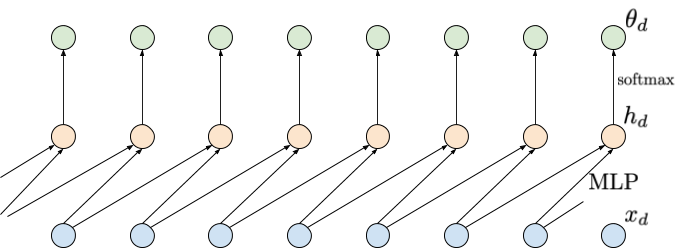
\includegraphics[width=0.5\linewidth]{figs/sequential_MLP}
		 \end{figure}
	\end{block}
	\vspace{-0.4cm}

	\begin{block}{Autoregressive transformer}
		\begin{minipage}[t]{0.5\columnwidth}
			\begin{figure}
				\centering
	      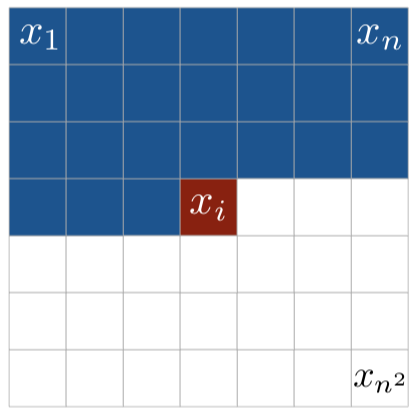
\includegraphics[width=0.6\linewidth]{figs/pixelcnn1}
			\end{figure}
		\end{minipage}%
		\begin{minipage}[t]{0.5\columnwidth}
			\vspace{-0.8cm}
			\begin{figure}
				\centering
		  			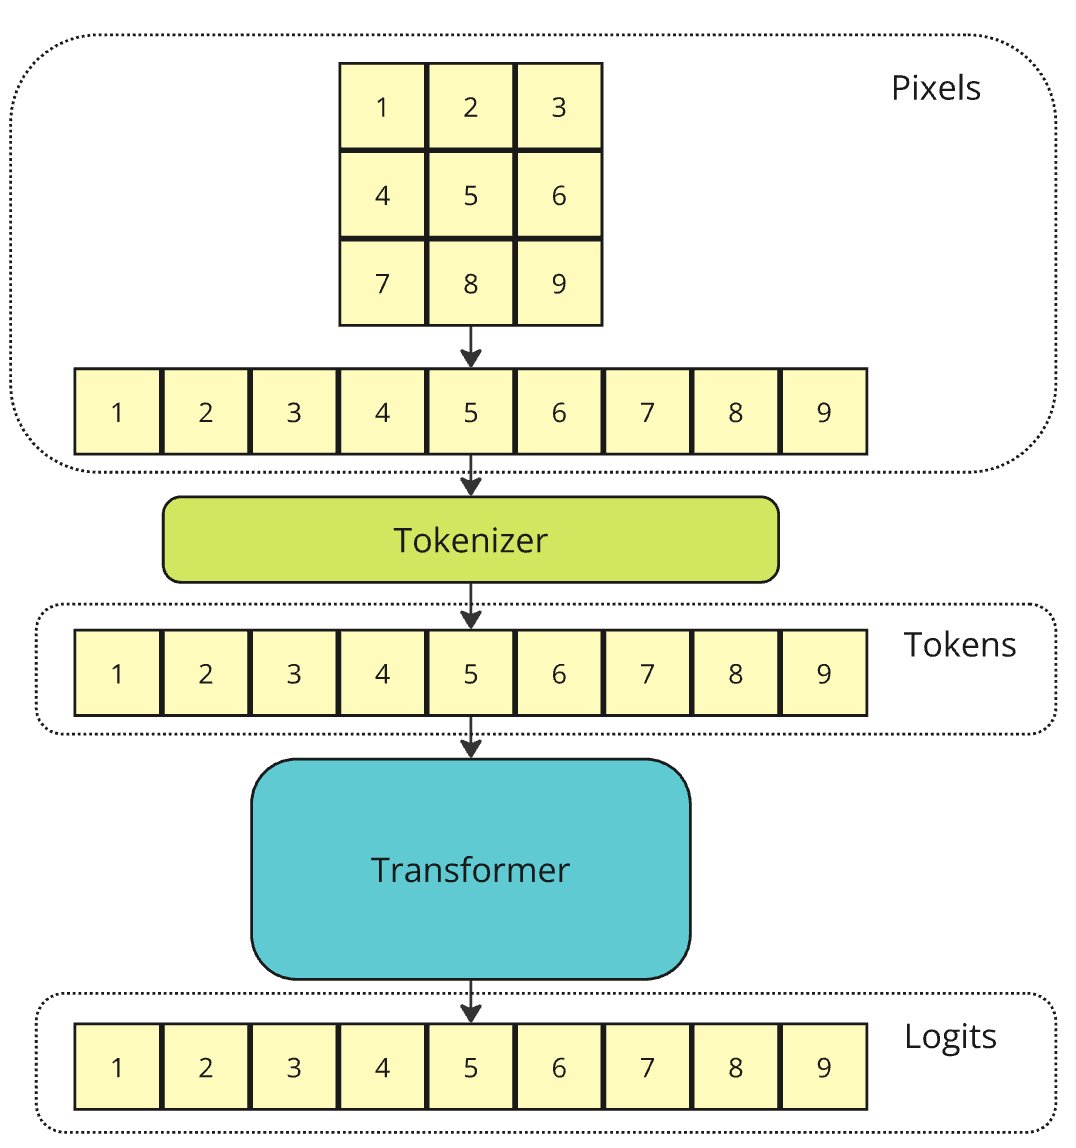
\includegraphics[width=0.8\linewidth]{figs/imagegpt.png}
			\end{figure}
		\end{minipage}
	\end{block}
	 \myfootnote{\href{https://jmtomczak.github.io/blog/2/2\_ARM.html}{image credit: https://jmtomczak.github.io/blog/2/2\_ARM.html}\\ \href{https://cdn.openai.com/papers/Generative_Pretraining_from_Pixels_V2.pdf}{Chen M. et al. Generative Pretraining from Pixels, 2020}}
\end{frame}
%=======
\begin{frame}{Outline}
	\tableofcontents
\end{frame}
%=======
\section{Normalizing flows (NF)}
%=======
\begin{frame}{Generative models zoo}
	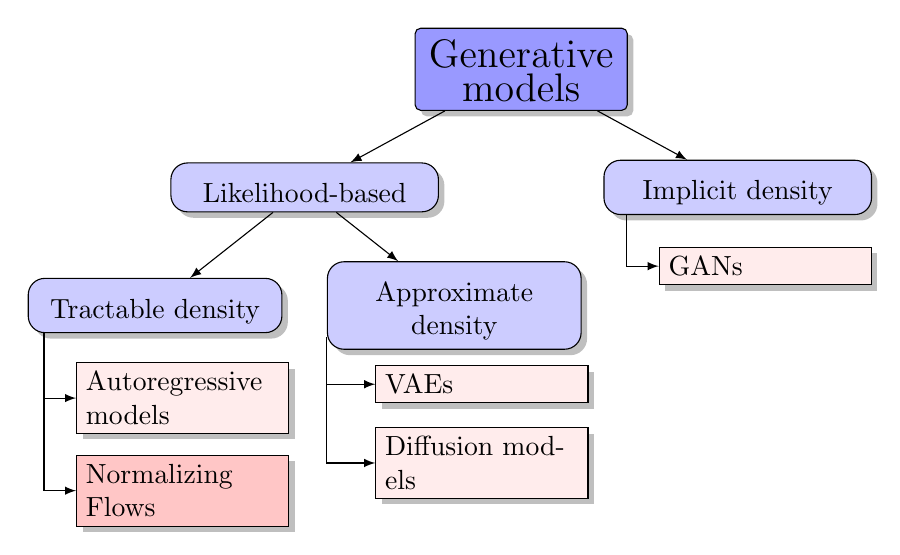
\begin{tikzpicture}[
	 	basic/.style  = {draw, text width=2cm, drop shadow, rectangle},
	 	root/.style   = {basic, rounded corners=2pt, thin, text height=1.1em, text width=7em, align=center, fill=blue!40},
	 	level 1/.style={sibling distance=55mm},
	 	level 2/.style = {basic, rounded corners=6pt, thin, align=center, fill=blue!20, text height=1.1em, text width=9em, sibling distance=38mm},
	 	level 3/.style = {basic, rounded corners=6pt, thin,align=center, fill=blue!20, text width=8.5em},
	 	level 4/.style = {basic, thin, align=left, fill=pink!30, text width=7em},
	 	level 5/.style = {basic, thin, align=left, fill=pink!90, text width=7em},
		edge from parent/.style={->,draw},
		>=latex]
		
		% root of the the initial tree, level 1
		\node[root] {\Large Generative models}
		% The first level, as children of the initial tree
		child {node[level 2] (c1) {Likelihood-based}
			child {node[level 3] (c11) {Tractable density}}
			child {node[level 3] (c12) {Approximate density}}
		}
		child {node[level 2] (c2) {Implicit density}};
		
		% The second level, relatively positioned nodes
		\begin{scope}[every node/.style={level 4}]
		\node [below of = c11, yshift=-5pt, xshift=10pt] (c111) {Autoregressive models};
		
		\node [below of = c12, xshift=10pt] (c121) {VAEs};
		\node [below of = c121] (c122) {Diffusion models};
		\node [below of = c2, xshift=10pt] (c21) {GANs};
		
		\end{scope}
		
		% The second level, relatively positioned nodes
		\begin{scope}[every node/.style={level 5}]
			\node [below of = c111, yshift=-5pt] (c112) {Normalizing Flows};
		\end{scope}
		
		
		% lines from each level 1 node to every one of its "children"
		\foreach \value in {1,2}
		\draw[->] (c11.194) |- (c11\value.west);
		
		\foreach \value in {1,2}
		\draw[->] (c12.194) |- (c12\value.west);
		
		\draw[->] (c2.194) |- (c21.west);
		
	\end{tikzpicture}
\end{frame}
%=======
\begin{frame}{Normalizing flows prerequisites}
	\begin{block}{Jacobian matrix}
		Let $\bff: \mathbb{R}^m \rightarrow \mathbb{R}^m$ be a differentiable function.
		\[
			\bz = \bff(\bx), \quad 
			\bJ =  \frac{\partial \bz}{\partial \bx} =
			\begin{pmatrix}
				\frac{\partial z_1}{\partial x_1} & \dots & \frac{\partial z_1}{\partial x_m} \\
				\dots & \dots & \dots \\ 
				\frac{\partial z_m}{\partial x_1} & \dots & \frac{\partial z_m}{\partial x_m}
			\end{pmatrix} \in \bbR^{m \times m}
		\]
		\vspace{-0.3cm}
	\end{block}
	\begin{block}{Change of variable theorem (CoV)}
		Let $\bx$ be a random variable with density function $p(\bx)$ and $\bff: \mathbb{R}^m \rightarrow \mathbb{R}^m$ is a differentiable, \textbf{invertible} function. If $\bz = \bff(\bx)$, $\bx = \bff^{-1}(\bz) = \bg(\bz)$, then
		\begin{align*}
			p(\bx) &= p(\bz) |\det(\bJ_{\bff})| = p(\bz) \left|\det \left( \frac{\partial \bz}{\partial \bx} \right) \right| = p(\bff(\bx)) \left|\det \left(  \frac{\partial \bff(\bx)}{\partial \bx} \right) \right| \\
			p(\bz) &= p(\bx) |\det(\bJ_{\bg})|= p(\bx) \left|\det \left(  \frac{\partial \bx}{\partial \bz} \right) \right| = p(\bg(\bz)) \left|\det \left(  \frac{\partial \bg(\bz)}{\partial \bz} \right) \right|.
		\end{align*}
		\vspace{-0.5cm}
	\end{block}
\end{frame}
%=======
\begin{frame}{Jacobian determinant}
	\begin{block}{Inverse function theorem}
		If function $\bff$ is invertible and Jacobian matrix is continuous and non-singular, then
		\vspace{-0.3cm}
		\[
		\bJ_{\bff^{-1}} = \bJ_{\bg} = \bJ_\bff^{-1}; \quad |\det (\bJ_{\bff^{-1}})| = |\det (\bJ_\bg)| = \frac{1}{|\det (\bJ_\bff)|}.
		\]
		\vspace{-0.3cm}
	\end{block}
	\begin{minipage}{0.55\columnwidth}
		\begin{itemize}
			\item $\bx$ and $\bz$ have the same dimensionality ($\bbR^m$).
			\vfill
			\item $\bff_{\btheta}(\bx)$ could be parametric function.
			\vfill
			\item Determinant  of Jacobian matrix $\mathbf{J} =\frac{\partial \bff_{\btheta}(\bx)}{\partial \bx}$ shows how the volume changes under the transformation.
		\end{itemize}
	\end{minipage}%
	\begin{minipage}{0.45\columnwidth}
		\begin{figure}
			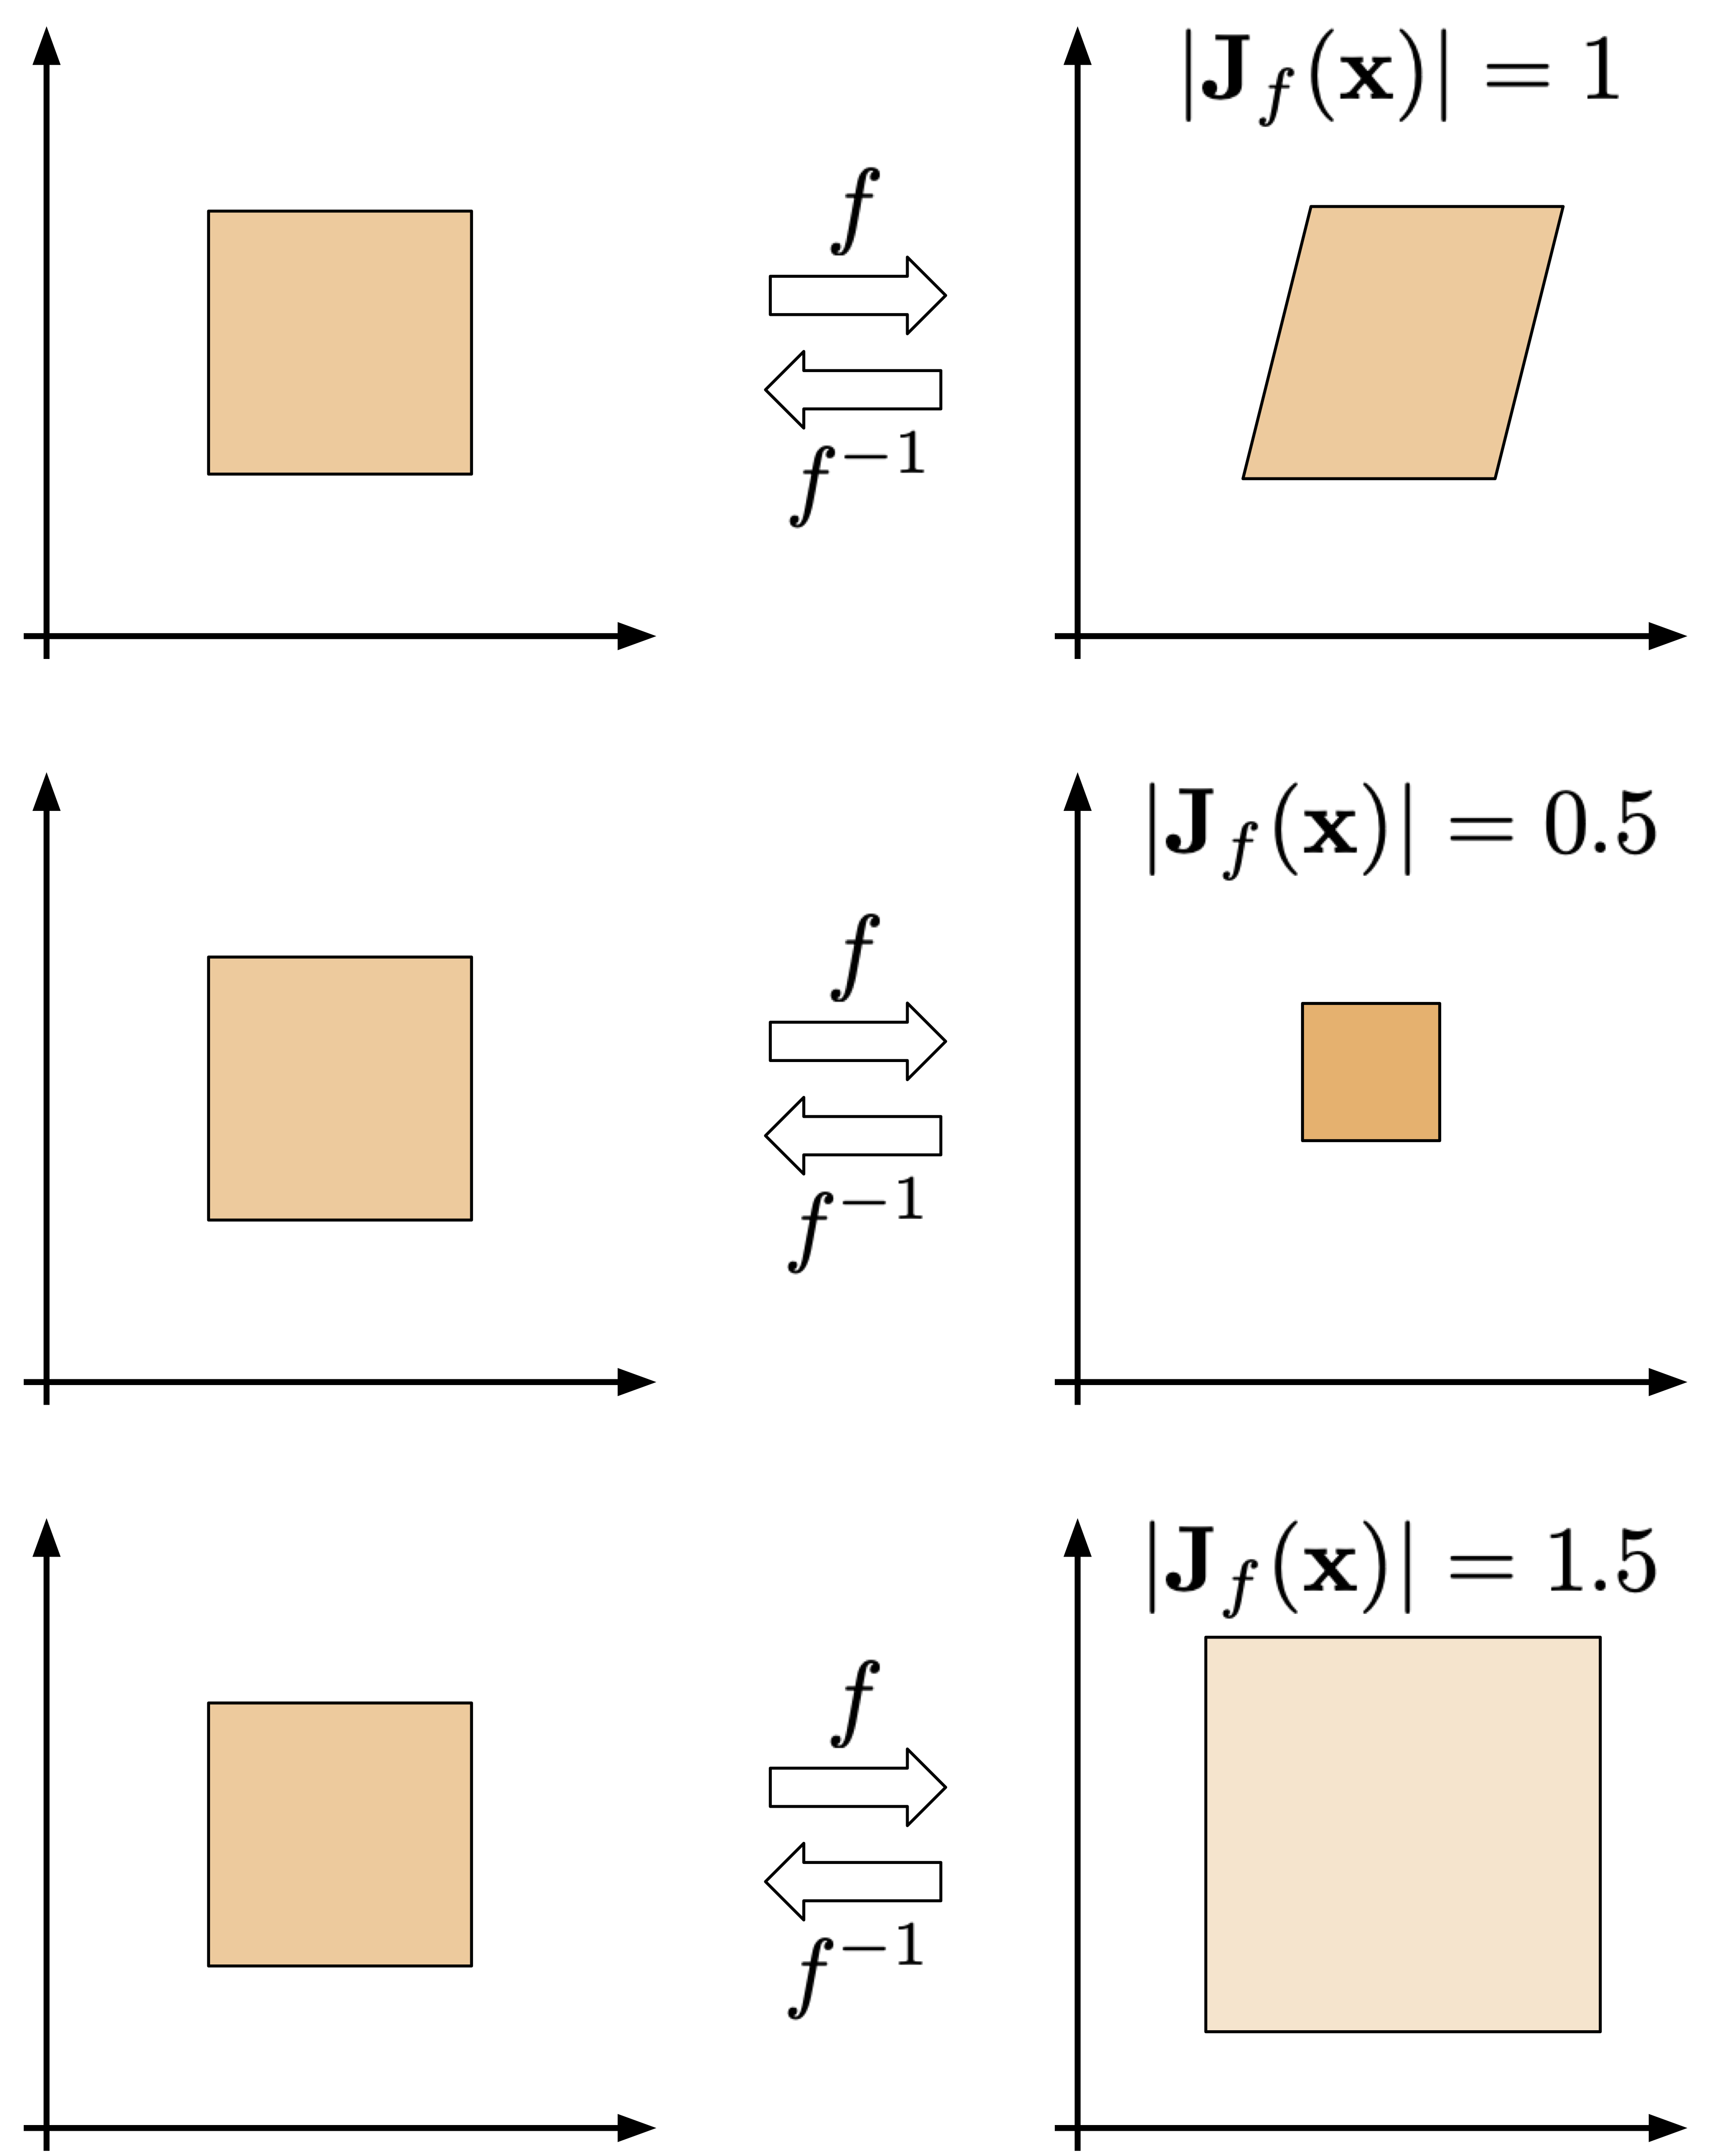
\includegraphics[width=0.8\linewidth]{figs/jacobian_det}
		\end{figure}
	\end{minipage}
	\myfootnotewithlink{https://jmtomczak.github.io/blog/3/3\_flows.html}{https://jmtomczak.github.io/blog/3/3\_flows.html}
\end{frame}
%=======
\begin{frame}{Fitting normalizing flows}
	\begin{block}{MLE problem}
		\vspace{-0.3cm}
		\[
		p(\bx|\btheta) = p(\bz) \left|\det \left(  \frac{\partial \bz}{\partial \bx} \right) \right|  = p(\bff_{\btheta}(\bx)) \left|\det \left( \frac{\partial \bff_{\btheta}(\bx)}{\partial \bx} \right) \right|
		\]
		\[
		\log p(\bx|\btheta) = \log p(\bff_{\btheta}(\bx)) + \log  |\det (\bJ_{\bff}) | \rightarrow \max_{\btheta}
		\]
	\end{block}
	\vspace{-0.2cm}
	\begin{figure}
		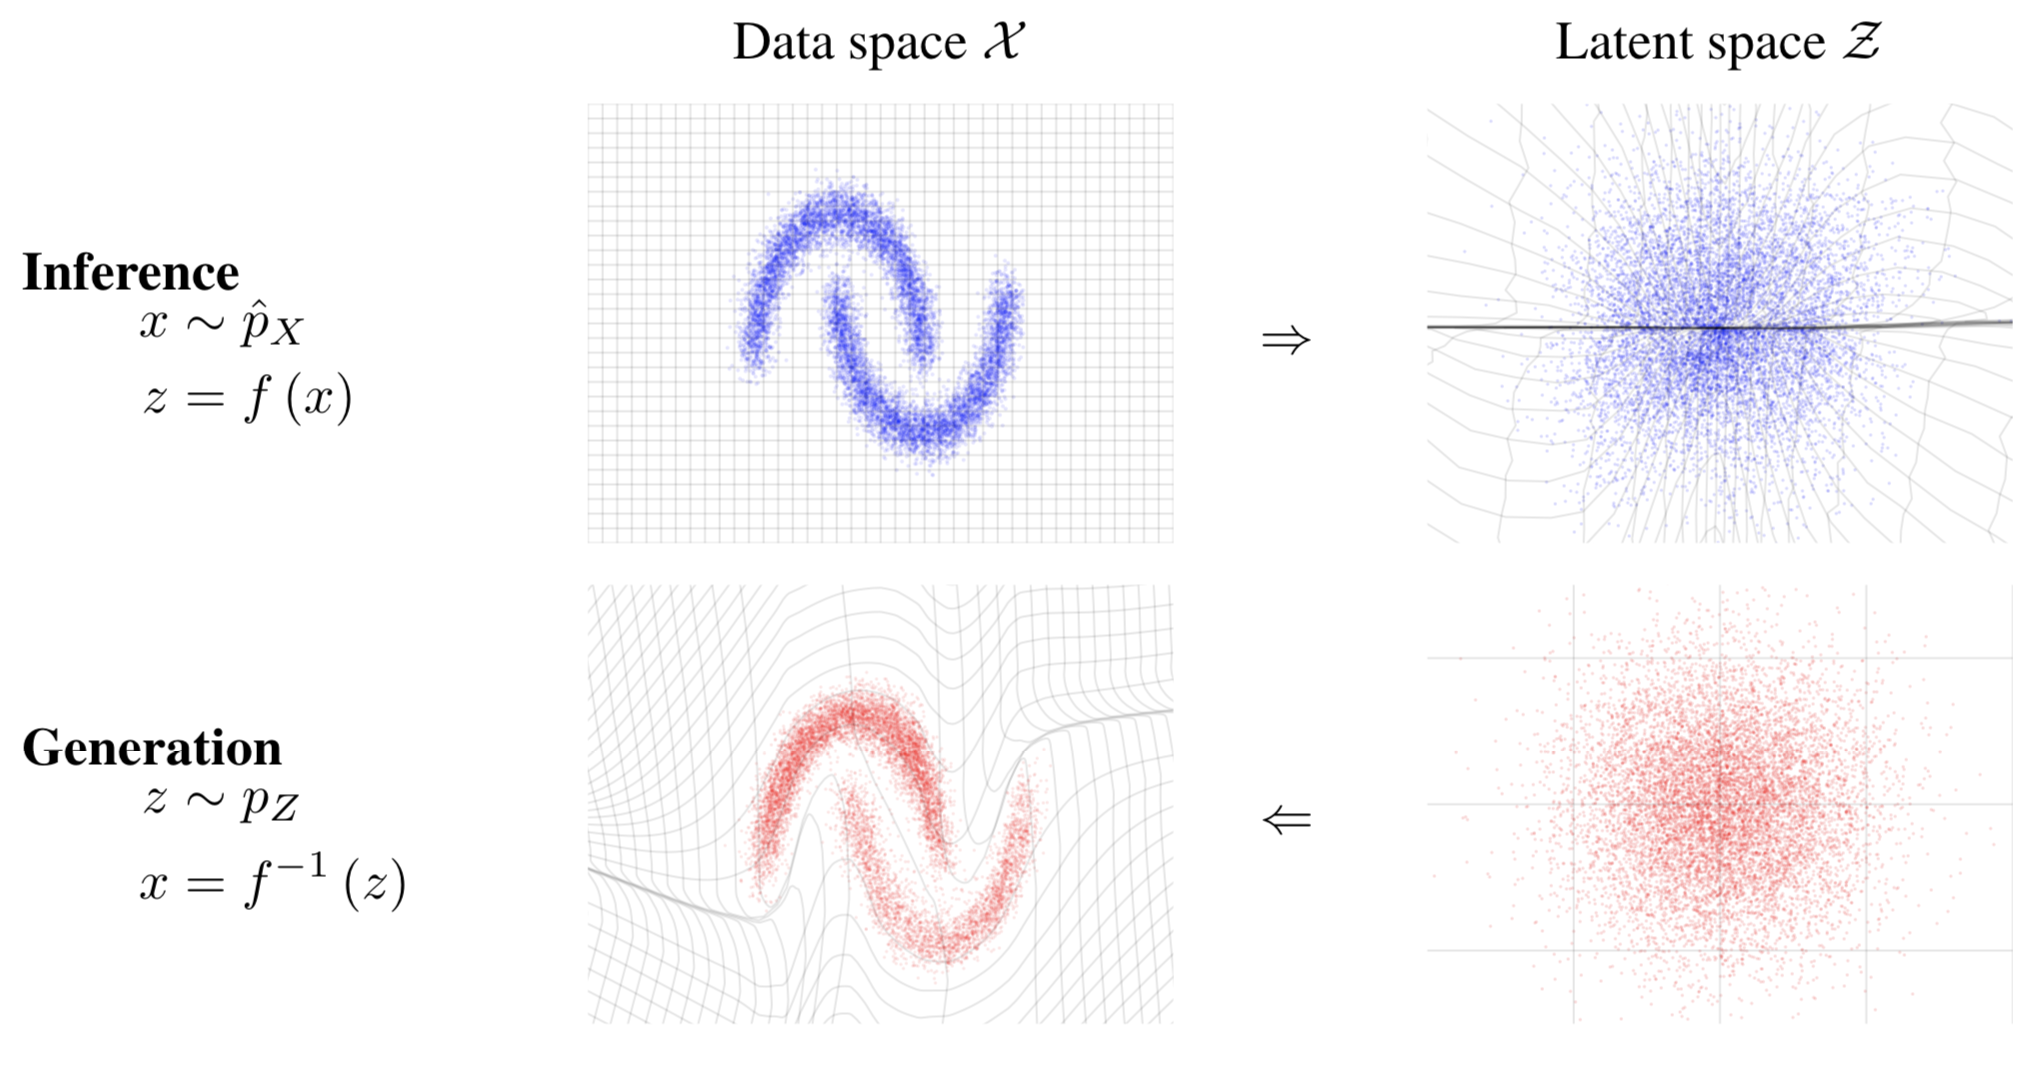
\includegraphics[width=0.85\linewidth]{figs/flows_how2}
	\end{figure}
	\myfootnotewithlink{https://arxiv.org/abs/1605.08803}{Dinh L., Sohl-Dickstein J., Bengio S. Density estimation using Real NVP, 2016} 
\end{frame}
%=======
\begin{frame}{Composition of normalizing flows}
	\vspace{-0.3cm}
	\begin{figure}
		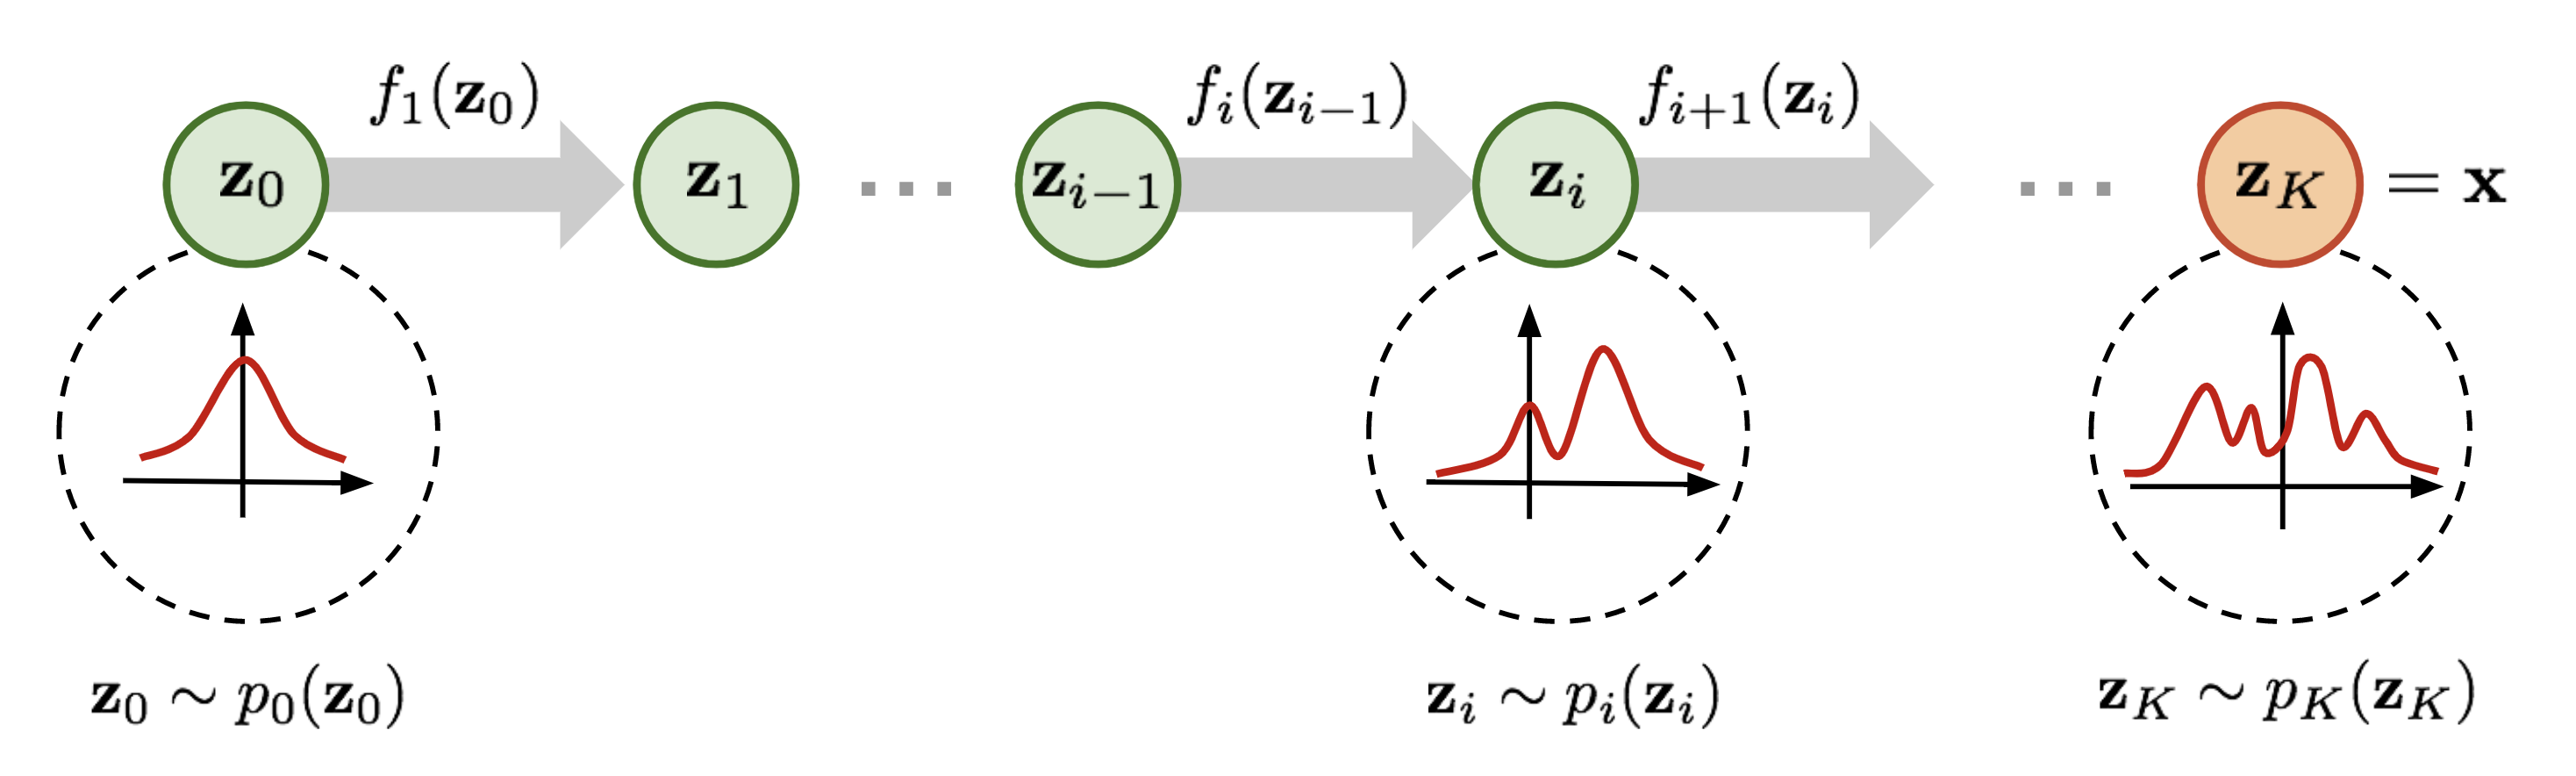
\includegraphics[width=0.95\linewidth]{figs/normalizing-flow}
	\end{figure}
	\vspace{-0.3cm}
	\begin{block}{Theorem}
		If $\{\bff_k\}_{k=1}^K$ satisfy conditions of the change of variable theorem, then $\bz = \bff(\bx) = \bff_K \circ \dots \circ \bff_1(\bx)$ also satisfies it.
	\end{block}
	\vspace{-0.5cm}
	{ \footnotesize
		\begin{multline*}
			p(\bx) = p(\bff(\bx)) \left|\det \left(\frac{\partial \bff(\bx)}{\partial \bx} \right) \right| =
			p(\bff(\bx)) \left|\det \left(\frac{\partial \textbf{f}_K}{\partial \textbf{f}_{K-1}} \dots \frac{\partial \textbf{f}_1}{\partial \bx} \right) \right| = \\ = p(\bff(\bx)) \prod_{k=1}^K \left|\det \left(\frac{\partial \textbf{f}_{k}}{\partial \textbf{f}_{k-1}} \right) \right|
			= p(\bff(\bx)) \prod_{k=1}^K |\det ( \bJ_{f_k}) |
		\end{multline*}
	}
	\myfootnotewithlink{https://lilianweng.github.io/lil-log/2018/10/13/flow-based-deep-generative-models.html}{https://lilianweng.github.io/lil-log/2018/10/13/flow-based-deep-generative-models.html}
\end{frame}
%=======
\begin{frame}{Normalizing flows (NF)}
	\vspace{-0.3cm}
	\[
	\log p(\bx|\btheta) = \log p(\bff_{\btheta}(\bx)) + \log |\det (\bJ_\bff)|
	\]
	\vspace{-0.4cm}
	\begin{block}{Definition}
		Normalizing flow is a \textit{differentiable, invertible} mapping from data $\bx$ to the noise $\bz$. 
	\end{block}
	\begin{itemize}
		\item \textbf{Normalizing} means that NF takes samples from $\pi(\bx)$ and normalizes them into samples from the base density $p(\bz)$.
		\item \textbf{Flow} refers to the trajectory followed by samples from $p(\bz)$ as they are transformed by the sequence of transformations
		\[
		\bz = \bff_K \circ \dots \circ \bff_1(\bx); \quad \bx = \bff_1^{-1} \circ \dots \circ \bff_K^{-1} (\bz) = \bg_1 \circ \dots \circ \bg_K(\bz) 
		\] 
		\vspace{-0.4cm}
		\begin{block}{Log likelihood}
			\vspace{-0.4cm}
			\[
			\log p(\bx | \btheta) = \log p(\bff_K \circ \dots \circ \bff_1(\bx)) + \sum_{k=1}^K\log |\det (\bJ_{\bff_k})|,
			\]
			\vspace{-0.4cm} \\
			where $\bJ_{\bff_k} = \frac{\partial \mathbf{f}_k}{\partial \bff_{k-1}}$.
		\end{block}
	\end{itemize}
	\textbf{Note:} Here we consider only \textbf{continuous} random variables.
\end{frame}
%=======
\begin{frame}{Normalizing flows}
	\begin{block}{Example of a 4-step NF}
		\vspace{-0.2cm}
		\begin{figure}
			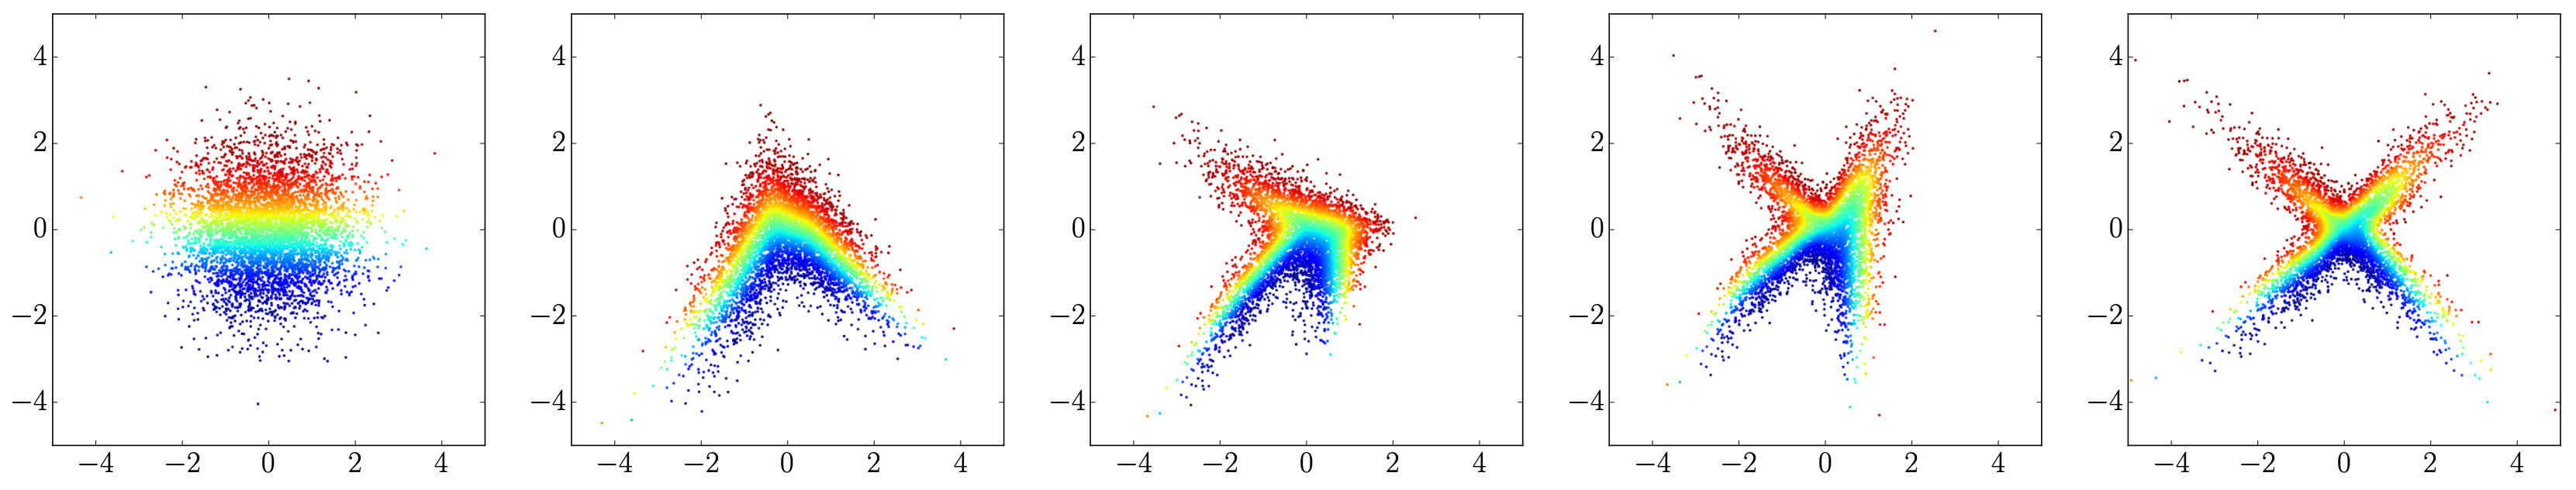
\includegraphics[width=\linewidth]{figs/flow_4_steps_example.png}
		\end{figure}
	\end{block}
	\vspace{-0.5cm}
	\begin{block}{NF log likelihood}
		\vspace{-0.3cm}
		\[
		\log p(\bx|\btheta) = \log p(\bff_{\btheta}(\bx)) + \log |\det ( \bJ_\bff)|
		\]
		\vspace{-0.3cm}
	\end{block}
	What is the complexity of the determinant computation?
	\begin{block}{What do we need?}
		\begin{itemize}
			\item efficient computation of the Jacobian matrix $\bJ_\bff = \frac{\partial \bff_{\btheta}(\bx)}{\partial \bx}$;
			\item efficient inversion of $\bff_{\btheta}(\bx)$.
		\end{itemize}
	\end{block}
	\myfootnotewithlink{https://arxiv.org/abs/1912.02762}{Papamakarios G. et al. Normalizing flows for probabilistic modeling and inference, 2019} 
\end{frame}
%=======
\section{NF examples}
%=======
\subsection{Linear normalizing flows}
%=======
\begin{frame}{Jacobian structure}
	\begin{block}{Normalizing flows log-likelihood}
		\[
			\log p(\bx|\btheta) = \log p(\bff_{\btheta}(\bx)) + \log \left|\det \left( \frac{\partial \bff_{\btheta}(\bx)}{\partial \bx} \right) \right|
		\]
	\end{block}
	The main challenge is a determinant of the Jacobian matrix.
	\begin{block}{What is the $det(\bJ)$ in the following cases?}
		Consider a linear layer $\bz = \bW \bx$, $\bW \in \bbR^{m \times m}$.
		\begin{enumerate}
			\item Let $\bz$ be a permutation of $\bx$. 
			\item Let $z_j$ depend only on $x_j$. 
			\[
				\log \left|\det \left( \frac{\partial \bff_{\btheta}(\bx)}{\partial \bx} \right) \right| = \log \left| \prod_{j=1}^m \frac{\partial f_{j, \btheta}(x_j)}{\partial x_j} \right| = \sum_{j=1}^m \log \left|  \frac{\partial f_{j, \btheta}(x_j)}{\partial x_j} \right|.
			\]
			\item Let $z_j$ depend only on $\bx_{1:j}$ (autoregressive dependency). 
		\end{enumerate}
	\end{block}
\end{frame}
%=======
\begin{frame}{Linear normalizing flows}
	\[
		\bz = \bff_{\btheta}(\bx) = \bW \bx, \quad \bW \in \bbR^{m \times m}, \quad \btheta = \bW, \quad \bJ_\bff = \bW^T
	\]
	In general, we need $O(m^3)$ to invert matrix.
	\begin{block}{Invertibility}
		\begin{itemize}
			\item Diagonal matrix $O(m)$.
			\item Triangular matrix $O(m^2)$.
			\item It is impossible to parametrize all invertible matrices.
		\end{itemize}
	\end{block}
	\begin{block}{Invertible 1x1 conv}
			
		$\mathbf{W} \in \mathbb{R}^{c \times c}$ -- kernel of 1x1 convolution with $c$ input and $c$ output channels.
		The computational complexity of computing or differentiating $\det (\mathbf{W})$ is $O(c^3)$.
		Cost to compute $\det (\mathbf{W})$ is $O(c^3)$. It should be invertible.
	\end{block}
	
	\myfootnotewithlink{https://arxiv.org/abs/1807.03039}{Kingma D. P., Dhariwal P. Glow: Generative Flow with Invertible 1x1 Convolutions, 2018} 
\end{frame}
%=======
\begin{frame}{Linear normalizing flows}
	\vspace{-0.5cm}
	\[
		\bz = \bff_{\btheta}(\bx) = \bW \bx, \quad \bW \in \bbR^{m \times m}, \quad \btheta = \bW, \quad \bJ_\bff = \bW^T
	\]
	\vspace{-0.7cm}
	\begin{block}{Matrix decompositions}
		\begin{itemize}
			\item \textbf{LU-decomposition}
			\[
				\bW = \mathbf{P} \bL \bU,
			\]
			where $\mathbf{P}$ is a permutation matrix, $\mathbf{L}$ is lower triangular with positive diagonal, $\mathbf{U}$ is upper triangular with positive diagonal.
			\item \textbf{QR-decomposition}
			\[
				\bW = \bQ \mathbf{R},
			\]
			where $\bQ$ is an orthogonal matrix, $\mathbf{R}$ is an upper triangular matrix with positive diagonal.
		\end{itemize}
	\end{block}

	Decomposition should be done only once in the beggining. Next, we fit decomposed matrices ($\bP/\bL/\bU$ or $\bQ/\bR$).

	\myfootnote{\href{https://arxiv.org/abs/1807.03039}{Kingma D. P., Dhariwal P. Glow: Generative Flow with Invertible 1x1 Convolutions, 2018}  \\
	\href{https://arxiv.org/abs/1901.11137}{Hoogeboom E., et al. Emerging convolutions for generative normalizing flows, 2019}
	}
\end{frame}
%=======
\subsection{Gaussian autoregressive NF}
%=======
\begin{frame}{Gaussian autoregressive model}
	Consider an autoregressive model
	\vspace{-0.3cm}
	{\small
		\[
		p(\bx | \btheta) = \prod_{j=1}^m p(x_j | \bx_{1:j - 1}, \btheta), \quad
		p(x_j | \bx_{1:j - 1}, \btheta) = \mathcal{N} \left(\mu_{j, \btheta}(\bx_{1:j-1}), \sigma^2_{j, \btheta} (\bx_{1:j-1})\right).
		\]
	}
	\vspace{-0.5cm}
	\begin{block}{Sampling}
		\vspace{-0.3cm}
		\[
		x_j = \sigma_{j, \btheta} (\bx_{1:j-1}) \cdot z_j + \mu_{j, \btheta}(\bx_{1:j-1}), \quad z_j \sim \mathcal{N}(0, 1).
		\]
		\vspace{-0.7cm}
	\end{block}
	\begin{block}{Inverse transform}
		\vspace{-0.3cm}
		\[
		z_j = \left(x_j - \mu_{j, \btheta}(\bx_{1:j-1}) \right) \cdot \frac{1}{\sigma_{j, \btheta} (\bx_{1:j-1}) }.
		\]
		\vspace{-0.4cm}
	\end{block}
	\begin{itemize}
		\item We have an \textbf{invertible} and \textbf{differentiable} transformation from $p(\bz)$ to $p(\bx | \btheta)$.
		\item It is an autoregressive (AR) NF with the base distribution $p(\bz) = \cN(0, \bI)$!
		\item Jacobian of such transformation is triangular!
	\end{itemize}
	\myfootnotewithlink{https://arxiv.org/abs/1606.04934}{Kingma D. P. et al. Improving Variational Inference with Inverse Autoregressive Flow, 2016} 
\end{frame}
%=======
\begin{frame}{Gaussian autoregressive NF}
	\vspace{-0.5cm}
	\begin{align*}
		\bx &= \bg_{\btheta}(\bz) \quad \Rightarrow \quad {\color{violet} x_j} = \sigma_{j, \btheta} ({\color{violet} \bx_{1:j-1}}) \cdot {\color{teal} z_j} + \mu_{j, \btheta}({\color{violet} \bx_{1:j-1}}). \\
		\bz &= \bff_{\btheta}(\bx) \quad \Rightarrow \quad {\color{teal} z_j} = \left({\color{violet}x_j} - \mu_{j, \btheta}({\color{violet}\bx_{1:j-1}}) \right) \cdot \frac{1}{ \sigma_{j, \btheta} ({\color{violet}\bx_{1:j-1}})}.
	\end{align*}
	Generation function $\bg_{\btheta}(\bz)$ is \textbf{sequential}. \\ Inference function $\bff_{\btheta}(\bx)$ is \textbf{not sequential}.

	\begin{block}{Forward KL for NF}
		\vspace{-0.2cm}
		\[
			KL(\pi || p)  = - \bbE_{\pi(\bx)} \left[\log p(\bff_{\btheta}(\bx)) + \log  |\det (\bJ_\bff)|\right] + \text{const} 
		\]
		\vspace{-0.5cm}
		\begin{itemize}
			\item We need to be able to compute $\bff_{\btheta}(\bx)$ and its Jacobian.
			\item We need to be able to compute the density $p(\bz)$.
			\item We don’t need to think about computing the function $\bg_{\btheta}(\bz) = \bff_{\btheta}^{-1}(\bz)$ until we want to sample from the model.
		\end{itemize}
	\end{block}
	\myfootnotewithlink{https://arxiv.org/abs/1705.07057}{Papamakarios G., Pavlakou T., Murray I. Masked Autoregressive Flow for Density Estimation, 2017} 
\end{frame}
%=======
\begin{frame}{Gaussian autoregressive NF}
	\vspace{-0.5cm}
	\begin{align*}
		\bx &= \bg_{\btheta}(\bz) \quad \Rightarrow \quad {\color{violet} x_j} = \sigma_{j, \btheta} ({\color{violet} \bx_{1:j-1}}) \cdot {\color{teal} z_j} + \mu_{j, \btheta}({\color{violet} \bx_{1:j-1}}). \\
		\bz &= \bff_{\btheta}(\bx) \quad \Rightarrow \quad {\color{teal} z_j} = \left({\color{violet}x_j} - \mu_{j, \btheta}({\color{violet}\bx_{1:j-1}}) \right) \cdot \frac{1}{ \sigma_{j, \btheta} ({\color{violet}\bx_{1:j-1}})}.
	\end{align*}
	
	\begin{itemize}
		\item Sampling is sequential, density estimation is parallel.
		\item Forward KL is a natural loss.
	\end{itemize}
	\vspace{-0.3cm}
	
	\begin{minipage}[t]{0.65\columnwidth}
		\begin{block}{Forward transform: $\bff_{\btheta}(\bx)$}
			\[
				z_j = (x_j - \mu_{j, \btheta}(\bx_{1:j-1})) \cdot \frac{1}{\sigma_{j, \btheta} (\bx_{1:j-1}) }
			\]
			\vspace{-0.4cm}
		\end{block}
	\end{minipage}% 
	\begin{minipage}[t]{0.35\columnwidth}
		\begin{figure}[h]
			\centering
			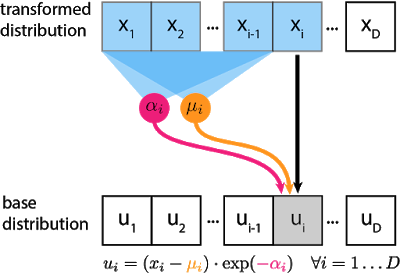
\includegraphics[width=.9\linewidth]{figs/af_iaf_explained_2.png}
		\end{figure}
	\end{minipage} \\
	
	\begin{minipage}[t]{0.65\columnwidth}
		\begin{block}{Inverse transform: $\bg_{\btheta}(\bz)$}
			\[
			x_j = \sigma_{j, \btheta} (\bx_{1:j-1}) \cdot z_j + \mu_{j, \btheta}(\bx_{1:j-1})
			\]
		\end{block}
	\end{minipage}%
	\begin{minipage}[t]{0.35\columnwidth}
		\begin{figure}[h]
			\centering
			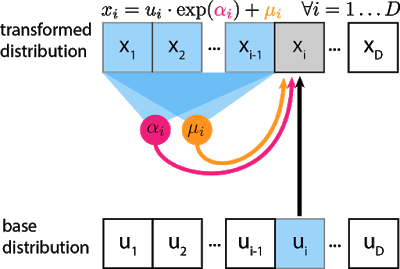
\includegraphics[width=.9\linewidth]{figs/af_iaf_explained_1.png}
		\end{figure}
	\end{minipage}
	\myfootnotewithlink{https://blog.evjang.com/2018/01/nf2.html}{image credit: https://blog.evjang.com/2018/01/nf2.html}
\end{frame}
%=======
\subsection{Coupling layer (RealNVP)}
%=======
\begin{frame}{RealNVP}
	\vspace{-0.5cm}
	Let split $\bx$ and $\bz$ in two parts: 
	\[
		\bx = [\bx_1, \bx_2] = [\bx_{1:d}, \bx_{d+1:m}]; \quad \bz = [\bz_1, \bz_2] = [\bz_{1:d}, \bz_{d+1:m}].
	\]
	\vspace{-0.7cm}
	\begin{block}{Coupling layer}
		\vspace{-0.7cm}
		\[
			\begin{cases} \bx_1 = \bz_1; \\ \bx_2 = \bz_2 \odot \bsigma_{\btheta}(\bz_1) + \bmu_{\btheta}(\bz_1).\end{cases}  
			\begin{cases} \bz_1 = \bx_1; \\ \bz_2 = \left(\bx_2 - \bmu_{\btheta}({\color{olive}\bx_1}) \right) \odot \frac{1}{\bsigma_{\btheta}({\color{olive}\bx_1})}.\end{cases}
		\]
	\end{block}
	\vspace{-0.5cm}
	\begin{block}{Image partitioning}
		
		\begin{minipage}[t]{0.5\columnwidth}
			\begin{figure}
				\centering
				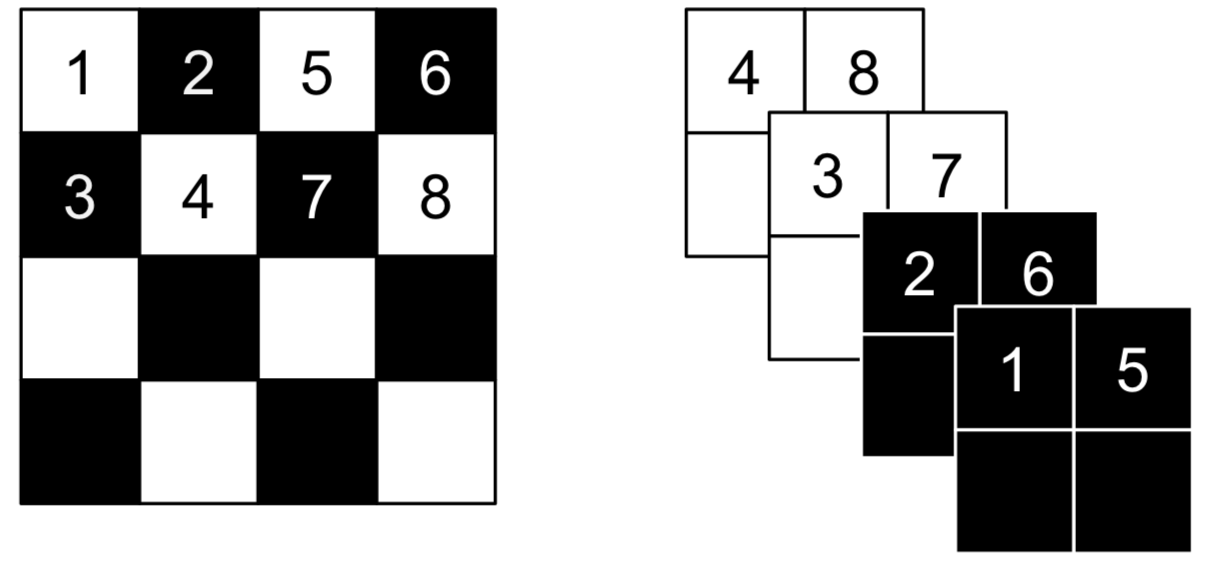
\includegraphics[width=\linewidth]{figs/realnvp_masking.png}
			\end{figure}
		\end{minipage}% 
		\begin{minipage}[t]{0.5\columnwidth}
			\begin{itemize}
				\item Checkerboard ordering uses masking.
				\item Channelwise ordering uses splitting.
			\end{itemize}
		\end{minipage}
	\end{block}
	\vspace{-0.5cm}
	\myfootnotewithlink{https://arxiv.org/abs/1605.08803}{Dinh L., Sohl-Dickstein J., Bengio S. Density estimation using Real NVP, 2016} 
\end{frame}
%=======
\begin{frame}{RealNVP}
	\begin{block}{Coupling layer}
		\vspace{-0.7cm}
		\[
		 \begin{cases} {\color{violet}\bx_1} = {\color{teal}\bz_1}; \\ {\color{violet}\bx_2} = {\color{teal}\bz_2} \odot \bsigma_{\btheta}({\color{teal}\bz_1}) + \bmu_{\btheta}({\color{teal}\bz_1}).\end{cases}  
		\begin{cases} {\color{teal}\bz_1} ={\color{violet} \bx_1}; \\ {\color{teal}\bz_2} = \left({\color{violet}\bx_2} - \bmu_{\btheta}({\color{violet}\bx_1}) \right) \odot \frac{1}{\bsigma_{\btheta}({\color{violet}\bx_1})}.\end{cases}
		\]
		Estimating the density takes 1 pass, sampling takes 1 pass!
	\end{block}
	\begin{block}{Jacobian}
		\vspace{-0.5cm}
		\[
		\det \left( \frac{\partial \bz}{\partial \bx} \right) = \det 
		\begin{pmatrix}
			\bI_d & 0_{d \times m - d} \\
			\frac{\partial \bz_2}{\partial \bx_1} & \frac{\partial \bz_2}{\partial \bx_2}
		\end{pmatrix} = \prod_{j=1}^{m - d} \frac{1}{\sigma_{j, \btheta}(\bx_1)}.
		\]
		\vspace{-0.5cm}
	\end{block}
	\begin{block}{Gaussian AR NF}
		\vspace{-0.6cm}
		\begin{align*}
			\bx &= \bg_{\btheta}(\bz) \quad \Rightarrow \quad {\color{violet}x_j} = \sigma_{j, \btheta} ({\color{violet}\bx_{1:j-1}}) \cdot {\color{teal} z_j} + \mu_{j, \btheta}({\color{violet}\bx_{1:j-1}}). \\
			\bz &= \bff_{\btheta}(\bx) \quad \Rightarrow \quad {\color{teal} z_j} = \left({\color{violet} x_j} - \mu_{j, \btheta}({\color{violet}\bx_{1:j-1}}) \right) \cdot \frac{1}{\sigma_{j, \btheta} ({\color{violet} \bx_{1:j-1}}) }.
		\end{align*}
		\vspace{-0.5cm}
	\end{block}
	How to get RealNVP coupling layer from gaussian AR NF?
	
	\myfootnotewithlink{https://arxiv.org/abs/1605.08803}{Dinh L., Sohl-Dickstein J., Bengio S. Density estimation using Real NVP, 2016} 
\end{frame}
%=======
\begin{frame}{Glow samples}
	Glow model: coupling layer + linear flows (1x1 convs)
	\begin{figure}
		\centering
		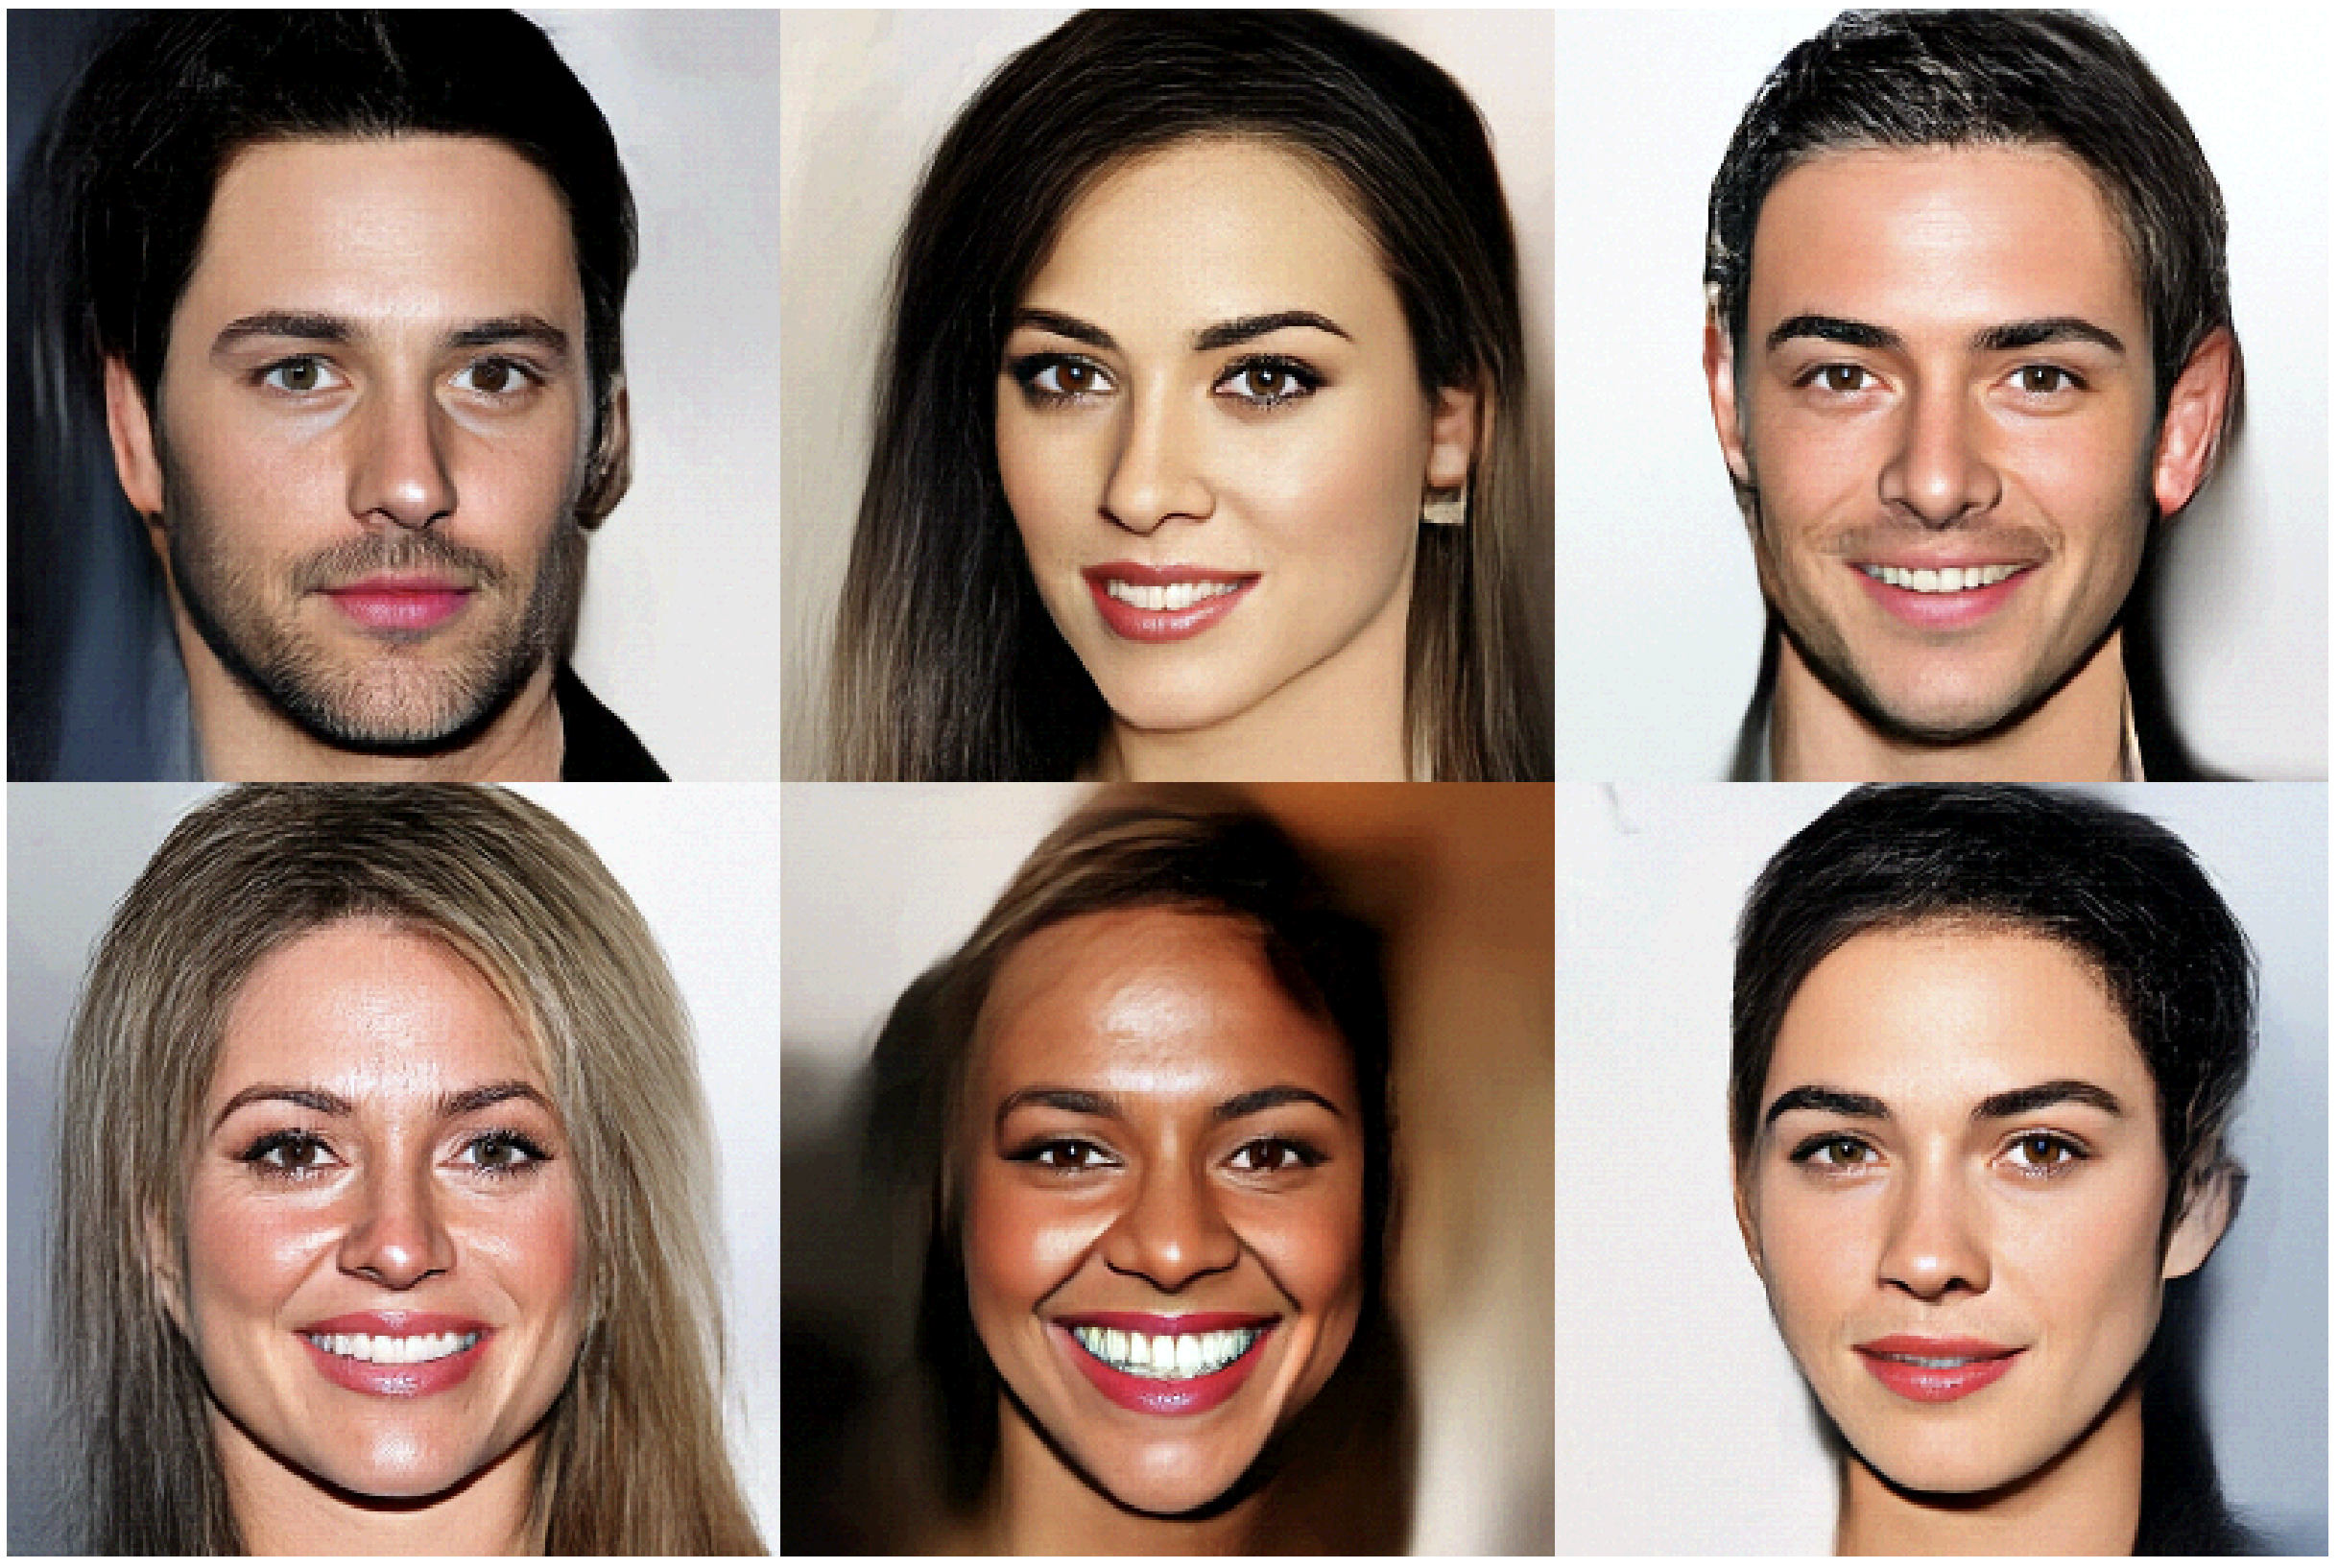
\includegraphics[width=0.9\linewidth]{figs/glow_faces.png}
	\end{figure}
	\myfootnotewithlink{https://arxiv.org/abs/1807.03039}{Kingma D. P., Dhariwal P. Glow: Generative Flow with Invertible 1x1 Convolutions, 2018}
\end{frame}
%=======
\begin{frame}{Summary}
	\begin{itemize}
		\item Change of variable theorem allows to get the density function of the random variable under the invertible transformation.
		\vfill
		\item Normalizing flows transform a simple base distribution to a complex one via a sequence of invertible transformations with tractable Jacobian.
		\vfill
		\item Normalizing flows have a tractable likelihood that is given by the change of variable theorem.
		\vfill
		\item Linear NF try to parametrize set of invertible matrices via matrix decompositions.
		\vfill
		\item Gaussian autoregressive NF is an autoregressive model with triangular Jacobian. 
		\vfill
		\item The RealNVP coupling layer is an effective type of NF (special case of AR NF) that has fast inference and generation modes.
	\end{itemize}
\end{frame}
\end{document} 